\documentclass[preview,border=5pt]{standalone}
\usepackage{teaching}
\begin{document}

\centering
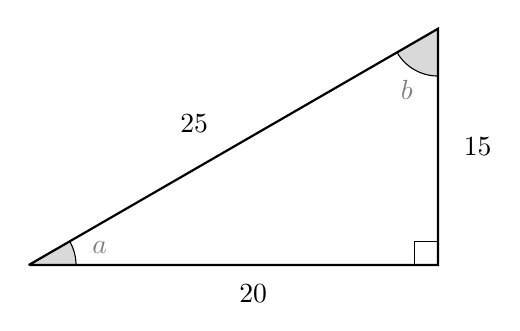
\begin{tikzpicture}[yscale=1,xscale=1,scale=6,inner sep=0.1mm, label distance=1.5mm]

\draw[fill=black!15!white] (0,0) -- (0.1,0) arc (0:30:0.1cm)  -- (0,0);
\draw[fill=black!15!white] (0.86602540378,0.5) -- (0.86602540378,0.4) arc (270:210:0.1cm)  -- (0.86602540378,0.5);
\draw[thick] (0,0) -- (0.86602540378,0.5) -- (0.86602540378,0) -- (0,0);

\node(t) at (0.15,0.0375) [color=black!50!white] {$a$};
\node(s) at (0.8,0.37) [color=black!50!white] {$b$};
\node(1) at (0.35,0.3) {$25$};
\node(0) at (0.475,-0.06) {$20$};
\node(2) at (0.95,0.25) {$15$};
\draw (0.86602540378,0) -- (0.81602540378,0) -- (0.81602540378,0.05) -- (0.86602540378,0.05);

\end{tikzpicture}
\end{document}
